\section{Radio Firmware and the Two-Board Stand}
\label{sec:radio}

The C implementation was measured first as a RAM-resident bench over
JTAG (Section~\ref{sec:cport_ontarget}); this section takes it the rest
of the way to a modem: two STM32H743 boards, each with its own crystal,
wired DAC to ADC, running a flash-resident image that is the whole
station --- PHY, link layer, carrier sense, broadcast --- with a host
attached over USB (Section~\ref{sec:host}).  The stand itself is
described as a channel in Section~\ref{sec:chan_wire}.

The order is chronological because the findings were: the first frame
across the wire, the firmware that made a board a radio, the streamed
bursts that failed on the boards and nowhere else, a sentinel that
crossed the air, the lessons a clean wire taught the broadcast
statistics exchange, and finally what the transfer levers of the
capability handshake (Section~\ref{sec:cport_caps}) were worth in
bytes per second.  Each subsection ends with the invariant the finding
left behind; the mechanisms themselves are specified in
Part~\ref{part:link} and Section~\ref{sec:cport}.

\subsection{Two Boards on a Wire}
\label{sec:cport_twoboard}

Everything to this point validated the chain against something the
project itself controls: golden vectors, a simulated channel, a virtual
audio daemon, and an SDR whose transmit and receive halves share one
oscillator. One impairment was never exercised by any of them --- two
\emph{independent} clocks. A single-board loopback cannot supply it
either: playing to \texttt{DAC1\_OUT1} and recording \texttt{ADC1} on
the same board runs both converters off one TIM6, so the sample-rate
offset is exactly zero by construction, and the receiver's tolerance to
it is untested no matter how much copper the signal crosses.

The stand in Figure~\ref{fig:twoboardlink} removes that last shared
assumption. Board A's DAC drives board B's ADC through one signal wire
and one ground wire; each board clocks its converter from its own
crystal and its own PLL, and the two never exchange a timing signal ---
not even to start. One ESP32 debugs both boards at once: JTAG
daisy-chains, so \texttt{TDI}/\texttt{TDO} thread through board A into
board B and back to the probe, which costs exactly one wire beyond a
second board's worth of the existing harness. The three push-pull
control lines are duplicated onto a driver pin per board rather than
spliced; because a line and its copy sit in the same GPIO bank, the
firmware switches both in one \texttt{w1ts}/\texttt{w1tc} store, so
there is no skew between the boards at all. That is a wiring
convenience rather than a fix: at the probe's measured 42\,236 edges/s
a TCK half-period is 25\,\textmu s, against nanoseconds of everything
else.

\begin{figure}[htbp]
    \centering
    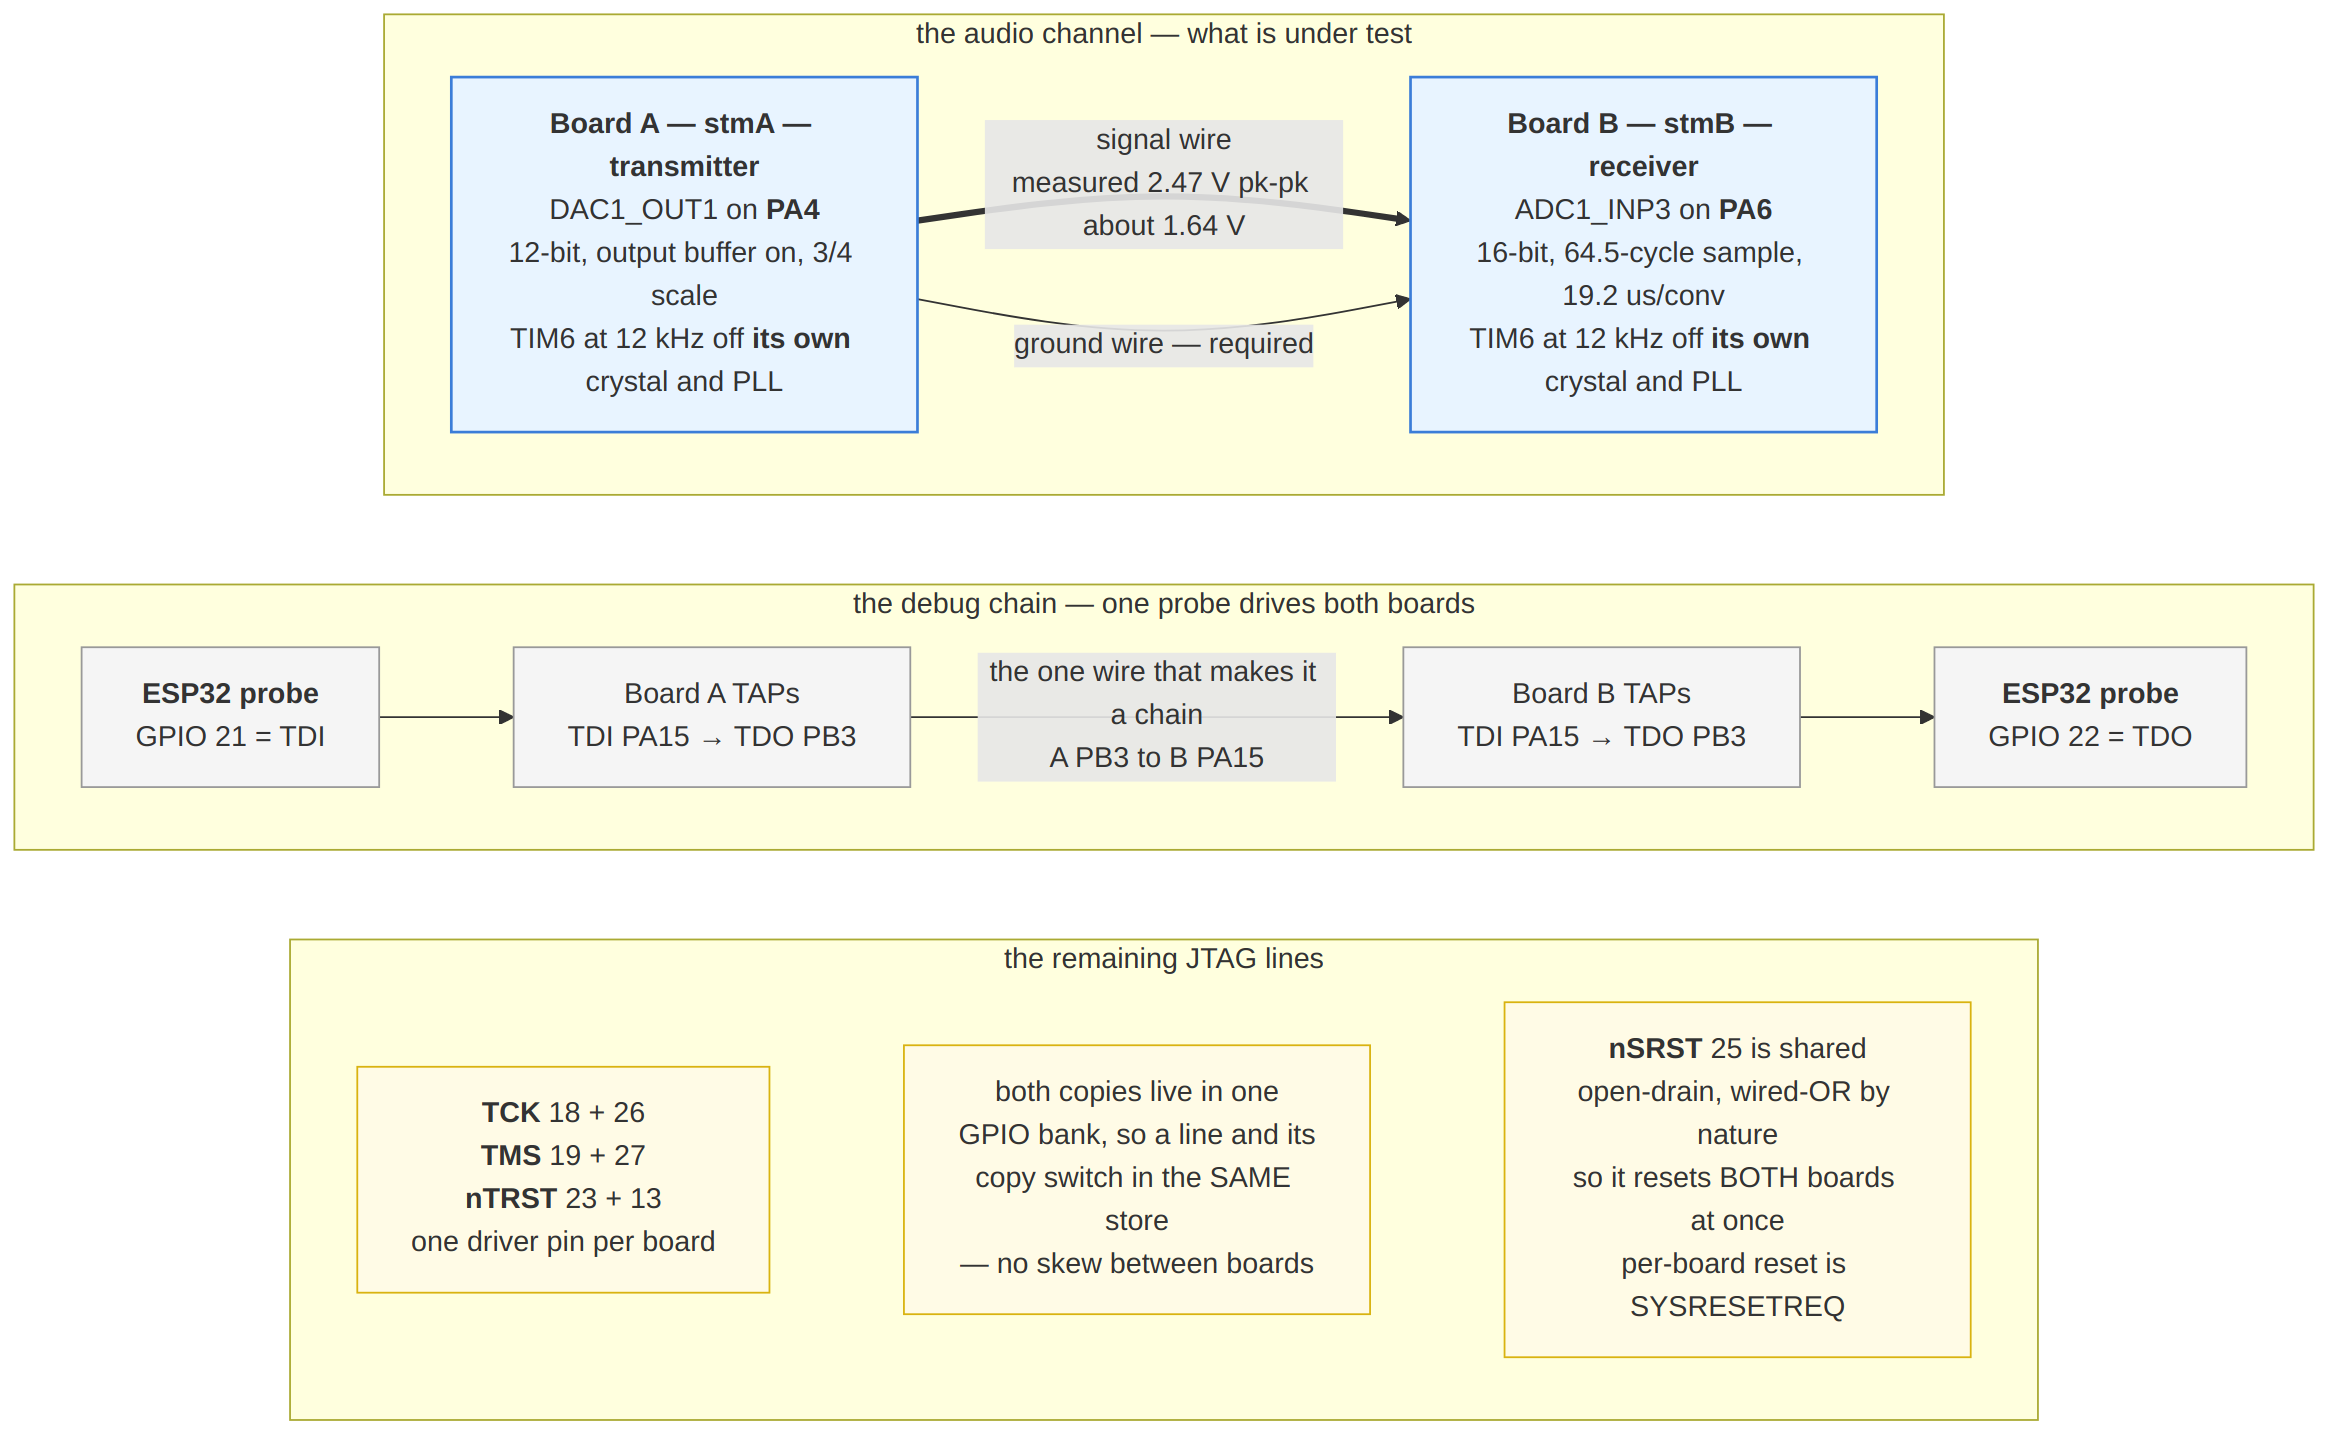
\includegraphics[width=\textwidth]{images/two_board_link.png}
    \caption{The two-board stand. The audio channel is one signal wire
             and one ground wire between converters that share no clock;
             the debug chain is a single probe threaded through both
             boards' TAPs. \texttt{nSRST} is deliberately not
             duplicated --- it is open-drain and wired-OR by nature, and
             duplicating it would not buy per-board reset anyway, since
             \texttt{remote\_bitbang} drives both resets from one pair of
             commands.}
    \label{fig:twoboardlink}
\end{figure}

One image serves both roles, selected over JTAG before the CPU is
released, because a station is half duplex and its transmitter shares
the receiver's arena --- no board ever does both. The transmitter builds
one NORMAL QPSK frame and replays it; the receiver records 54\,000
samples and only then runs the streaming receiver over the recording, so
the analog path can be characterised independently of whether the
decoder liked it. The host releases the transmitter \emph{first}, which
is what removes the need for a trigger: the whole capture window falls
inside a transmission already in progress.

\begin{table}[H]
    \centering
    \caption{Two boards, one wire, independent clocks. Measured on the
             stand; the payload check is \texttt{memcmp} against the
             transmitted packet, so ``bit-exact'' is exact.}
    \label{tab:twoboard}
    \small
    \begin{tabular}{@{}lll@{}}
    \toprule
    \textbf{Quantity} & \textbf{Measured} & \textbf{Note} \\
    \midrule
    Complete frames in window & 2 & 54\,000 samples at 12\,kHz \\
    Decoded bit-exact         & \textbf{2 of 2} & \texttt{memcmp} vs.\ the
                                                  transmitted packet \\
    ADC swing                 & 2.472\,V pk-pk & about 1.643\,V, the
                                                 DAC's mid-rail \\
    Residual CFO              & $+0.01$\,Hz & after preamble correction \\
    ADC conversion            & 19.2\,\textmu s & 64.5-cycle sample,
                                                  \texttt{per\_ck}/8 \\
    Receiver ISR              & 19.5\,\textmu s & of an 83.3\,\textmu s
                                                  period, i.e.\ 23\,\% \\
    Transmitter ISR           & 0.11\,\textmu s & one DAC store \\
    \bottomrule
    \end{tabular}
\end{table}

\paragraph{What it corrected: a vector table in cached SRAM.} The
receiver role hung on its first run --- stage ``running'', its TIM6
interrupt count stuck at zero, the run loop spinning until the
three-minute timeout. The state read off the part was contradictory:
TIM6 counting with its update flag set, the interrupt \emph{pending}
(\texttt{ISPR1}~$=$~\texttt{0x400000}) but \emph{not enabled}
(\texttt{ISER1}~$=$~0), \texttt{PRIMASK} clear --- and the vector table
in memory holding the correct handler. The status block explained the
disable: the first interrupt had been taken by the \emph{stray} handler,
whose job is to mask an unexpected source rather than let it wedge the
device, so it had cleared the enable for IRQ~54.

The vector table lives in ordinary cached SRAM, and
\texttt{vectors\_set()} wrote the entry and executed \texttt{DSB} ---
which orders accesses but does not clean. On a Cortex-M7 an exception
vector fetch reads \emph{memory}, not the D-cache, so the new entry sat
in a dirty line while the hardware still fetched the old one. Reading
the table over JTAG showed the correct handler only because the line had
been evicted by then, which is precisely what made the failure look
impossible. \texttt{SCB\_CCR} read \texttt{0x00070200} on the stalled
board, \texttt{DC} set --- inherited from the USB firmware the RAM image
had displaced. The transmitter role never hit it because
\texttt{build\_frame()} runs between installing the handler and the
first interrupt and evicts the line in time: the same binary on the same
board, differing only in eviction timing, which is why the bug presented
as role-dependent. Both entry points now clean by MVA. This had been
latent under every RAM bench in the project.

Two smaller hazards came from the same root --- a RAM image inherits the
machine state of the firmware it replaced. \texttt{ISER3} bit~5
(\texttt{OTG\_FS}) is still set when the image starts, so an inherited
enable can deliver a stale interrupt as the first one and get its source
masked; \texttt{vectors\_irq\_enable()} therefore clears the pending bit
before setting the enable, and the bench masks interrupts for the whole
of bring-up.

\paragraph{What was not measured.} The obvious way to report the
sample-rate offset --- compare the two boards' measured TIM6 clocks ---
is structurally incapable of showing it, and would have produced a
confident \emph{0.0\,ppm}. Each board measures TIM6 against its own DWT
cycle counter, and both are derived from the \emph{same} PLL, so that
ratio is exact on each board and identical between them however far
apart the crystals are. The offset is instead read off the wire, from
the spacing of consecutively decoded frames against the number of
samples transmitted between them. With only two complete frames in the
capture window the span is 17\,920 samples, and a start position good to
one sample makes that a \emph{bound} rather than a figure: the two
clocks agree to within $\pm$56\,ppm. That is consistent with the
$+0.01$\,Hz residual CFO, and it is enough to say the link decodes
across independent clocks --- but it is not a measurement of their
offset. A tighter number needs a much longer capture, which needs the
receiver to decode as it goes rather than into a buffer --- which the
radio firmware of the next subsection does, and whose
\texttt{burst\_repro} harness put the real offset near 5\,ppm
(\S\ref{sec:cport_burstdebug}).

\subsection{A Board That Is a Radio}
\label{sec:cport_radio}

Section~\ref{sec:cport_usb} gave the board an identity and a host
protocol, but bound the station to a \emph{stub} PHY: queues, rate
ladder, ARQ and reply timers all ran for real, and nothing reached the
air. Section~\ref{sec:cport_twoboard} gave the opposite half --- frames
crossing copper between two boards' converters --- with no link layer
above them and no host beside them. This section is the two in one
image: a board a host drives over USB and a peer hears over a wire.

\begin{figure}[htbp]
    \centering
    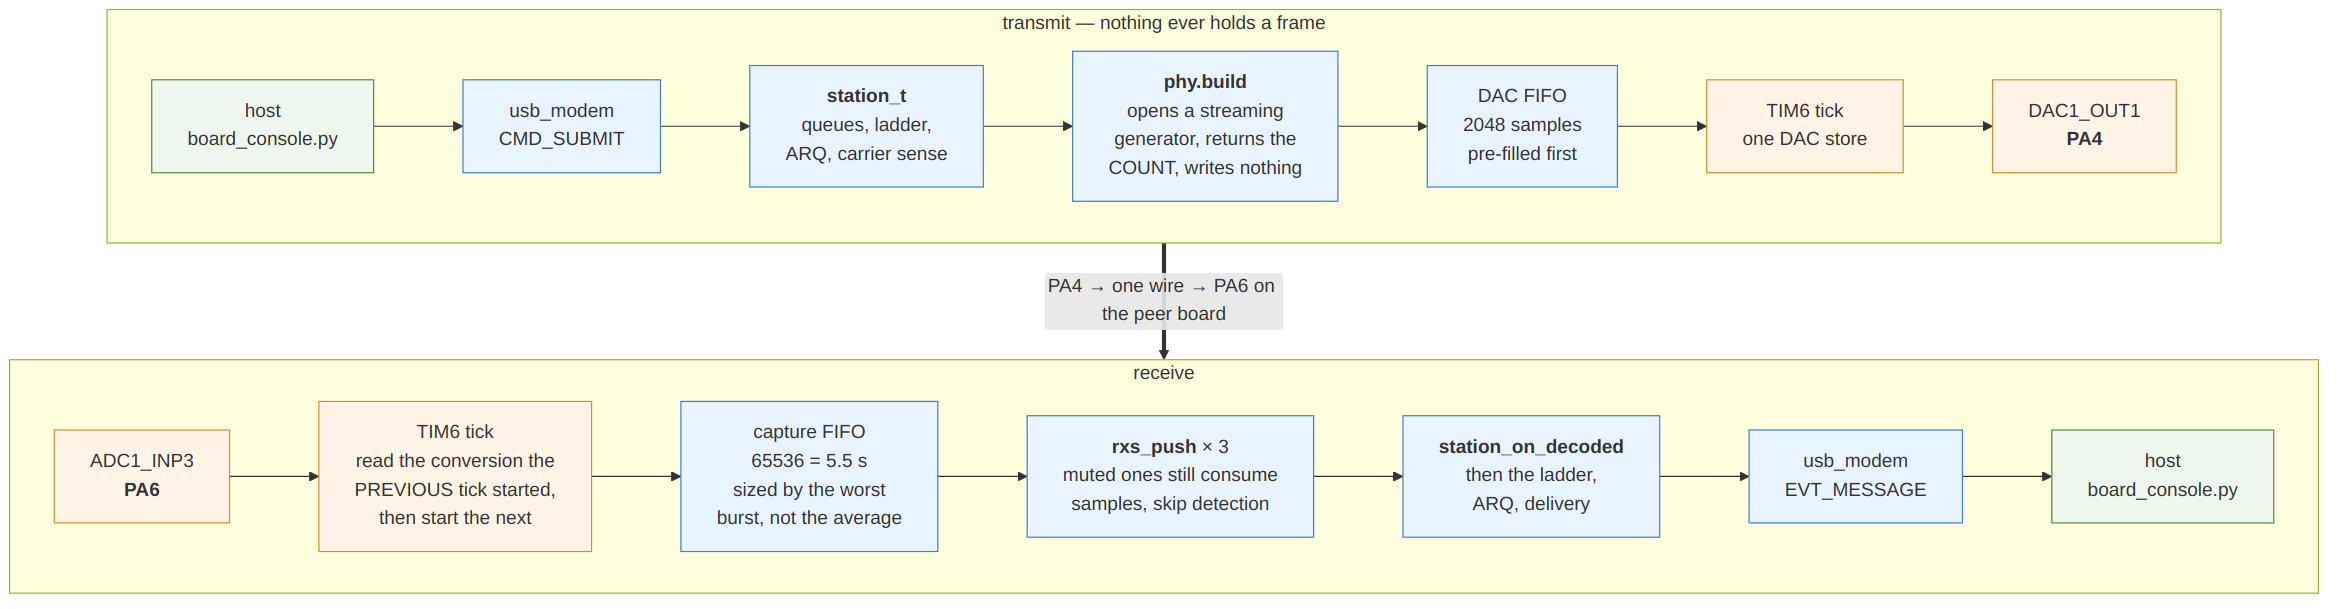
\includegraphics[width=\textwidth]{images/radio_firmware.png}
    \caption{The radio firmware. Half duplex here is a contract rather
             than a simplification: the streaming generator's state
             lives in the shared arena \emph{across} \texttt{txs\_pull}
             calls while the receiver's scratch is call-scoped, so
             \texttt{rxs\_push} must never run during a transmission ---
             and does not, because the tick feeds only one FIFO at a
             time.}
    \label{fig:radiofw}
\end{figure}

\paragraph{The transmitter never renders a frame.}
\texttt{station\_phy\_t::build} is frame-at-once: it is handed a buffer
and returns a sample count. An EXTREME frame is about 456\,000 samples
--- 912\,kB --- which this part cannot hold, and demoapp's answer (a
600\,000-sample buffer) is not available. It is also unnecessary. The
station never reads or writes those samples: \texttt{out} and
\texttt{out\_cap} appear nowhere in \texttt{station\_poll\_tx} except
where they are passed through to \texttt{build}, and the count is what
the caller acts on. So \texttt{build} here opens a \emph{streaming}
generator and returns the total it reports without writing a sample,
and the main loop pulls from that generator into a 2048-sample FIFO as
the tick drains it. The waveform is identical either way --- a one-block
burst with no resync is bit-for-bit a frame, which both test suites
already assert.

The 12\,kHz tick never blocks. The analog bench of
Section~\ref{sec:cport_twoboard} started a conversion and waited for it
inside the tick, 19.2\,\textmu s of an 83.3\,\textmu s period; that was
free when the decoder ran afterwards and is not free when the decoder
has to keep up. Here the tick reads the conversion the \emph{previous}
tick started and immediately starts the next, so the sample is one tick
old --- a constant delay indistinguishable from cable length.

\paragraph{What it corrected: the flash images never enabled the
caches.} The receiving board dropped 1\,522\,686 captured samples ---
64\,\% of everything its ADC produced --- and decoded nothing, while the
transmitting board underran its DAC 375 times. \texttt{SCB\_CCR} read
\texttt{0x00040200} on the running part: both L1 caches off.
\texttt{startup\_flash.c} had never enabled them, so code ran from flash
at two wait states with no instruction cache and every SRAM access
uncached, which is five to ten times slower than the same code out of
ITCM. It had not mattered while the flash images only ran a USB endpoint
and a link layer, and the RAM benches never showed it because their
\texttt{.text} lives in ITCM and needs no cache. Enabling both (the data
cache invalidated by set/way first) cut overruns by 61$\times$. Two
consequences follow and are handled rather than discovered later: a
debugger reading over the AHB-AP does \emph{not} see dirty lines, so the
beacon is cleaned explicitly before each read; and a RAM image that now
inherits \texttt{DC}=1 needs its vector-table writes cleaned, which is
what Section~\ref{sec:cport_twoboard} already had to fix.

Three smaller faults surfaced with it. The flash linker script listed
\texttt{.bss} \emph{before} \texttt{.d2\_bss}, and \texttt{.bss}'s
\texttt{*(.bss*)} matches \texttt{.bss.g\_raw} too --- so the D2 lines
matched nothing, the 160\,kB sample ring sat in AXI, and adding the
receiver overflowed AXI by 100\,kB while D2 stood completely empty
(\texttt{stm32h743\_usb.ld} always had the right order, which is why only
the flash images were affected). \texttt{TIM6\_DAC}, IRQ~54, had no entry
in the vector table: designated initialisers leave every other slot
\texttt{NULL}, so the first tick would have vectored to address zero.
And arming an empty DAC FIFO underran it once per transmission ---
166 underruns across 3 frames, each one a mid-rail sample on the air ---
which pre-filling before starting the carrier reduces to zero.

\paragraph{Sizing the capture FIFO: the worst burst, not the average.}
The decoder's cost is wildly uneven. Quiet blocks are cheap; the commit
at the end of a frame --- acquisition, demodulation of every tiled
symbol, Viterbi --- is one long blocking call, measured at 2283\,ms
inside a single \texttt{rxs\_push} against a 19.5\,s frame. As an
average that is about 12\,\% duty, comfortably real time. What matters
is not the average but whether the FIFO can hold the samples that keep
arriving \emph{through} the burst: 16\,384 samples (1.37\,s) could not,
dropping 33\,036 samples mid-frame and decoding nothing, while 65\,536
(5.5\,s) decodes with no overruns at all. The beacon carries
\texttt{cap\_overruns} and \texttt{push\_ms\_max} so this is checked on
the part rather than reasoned about.

\paragraph{The receiver follows the negotiated rung.} Each open receiver
runs its own detector over every sample and the EXTREME one is much the
most expensive; three concurrently do not fit real time on this part.
They cannot simply be opened selectively either, because every instance
shares one raw sample ring and indexes it by its \emph{own} sample
counter --- feed a subset and they write each other's history at the
wrong offsets. So all three are opened and the unwanted ones are
\emph{muted}: a muted instance still consumes every sample, keeping the
ring and its own timeline coherent, and skips only the per-block
detection, which is where the cost is. Unmuting rearms the search rather
than resuming, since a state machine that was mid-frame when it went
quiet would otherwise decode a frame whose middle it never saw.

Which are active follows \texttt{ladder\_mode(ctl.my\_req)} --- the rung
\emph{this} station asked the peer to transmit at --- plus two others
that are not optional. EXTREME always, because it is rung~0 and
therefore the bootstrap, it is where the ladder decays to after a spell
of silence, and it is what a peer that cannot hear us falls back to;
muting it would make the link undiscoverable and unrecoverable exactly
when recovery is needed. And the mode last decoded on, because
\texttt{my\_req} is a request rather than an observation: between raising
it and the peer acting on it, the peer is still transmitting at the old
mode, and dropping that mode immediately would make the station deaf for
precisely the exchange that would have confirmed the change --- timeout,
request decays, link oscillates. In the settled bootstrap state, both
terms are EXTREME and exactly one detector runs.

\begin{table}[H]
    \centering
    \caption{Two boards, one wire, driven from two host consoles. Every
             figure read off the boards' beacons or the consoles.}
    \label{tab:radio}
    \small
    \begin{tabular}{@{}lll@{}}
    \toprule
    \textbf{Quantity} & \textbf{Measured} & \textbf{Note} \\
    \midrule
    First message, end to end & 36\,s & EXTREME bootstrap,
                                        $\approx$19.5\,s of air \\
    Second message            & \textbf{15\,s} & after the ladder
                                                 climbed \\
    Frames / decodes, each board & 1 / 1 & B decoded, replied, A decoded
                                           the reply \\
    Capture overruns          & \textbf{0} & both boards, throughout \\
    DAC underruns             & \textbf{0} & both boards, after
                                             pre-filling \\
    Worst single decode       & 2283\,ms & of a 19.5\,s frame,
                                           $\approx$12\,\% duty \\
    Idle listening set        & EXTREME & \texttt{my\_req} 0, one
                                          detector \\
    After the climb           & NORMAL$+$EXTREME & \texttt{my\_req} 9
                                                   (A), 7 (B) \\
    SNR reported              & $+15.0$ / $+9.7$\,dB & A and B \\
    \bottomrule
    \end{tabular}
\end{table}

Streamed bursts --- a whole selective-repeat window behind one
preamble --- are the one part of the link this section does not settle:
their first implementation on the boards failed in a way that every
plausible theory misdiagnosed, and finding out why is a story worth a
subsection of its own.

\subsection{Debugging the Streamed Bursts}
\label{sec:cport_burstdebug}

The streaming continuation itself is small: after a decoded block whose
packet carries the link layer's streamed marker, the receiver takes the
next block from the deterministic offset past this one instead of
hunting for a preamble, and stops on the ack-request bit of the last
block. (\texttt{phy.receive\_burst} stays \texttt{NULL} by design ---
the station only reaches it from the frame-at-once \texttt{receive}
path, which is handed a whole recording this firmware never has.) The
same machinery passes every host test and runs demoapp's transfers. On
the boards it failed totally: block~0 of a stream decoded, and
\emph{every} continued block failed its data CRC, on every attempt, at
every rung --- while the same file crossed byte-exact as per-frame
fragments.

The failure looked exactly like a channel problem, and the two boards
are the first stand in the project where the two ends share no sample
clock --- so clock drift was the obvious suspect, with quantization
noise and the resync geometry close behind. All of it was wrong, and
what kept the search honest was the discipline in
Figure~\ref{fig:burstdebug}: reproduce on the \emph{host} first, where
a cycle costs seconds against the seven minutes of a
build--flash--transfer round on the boards.

\begin{figure}[htbp]
    \centering
    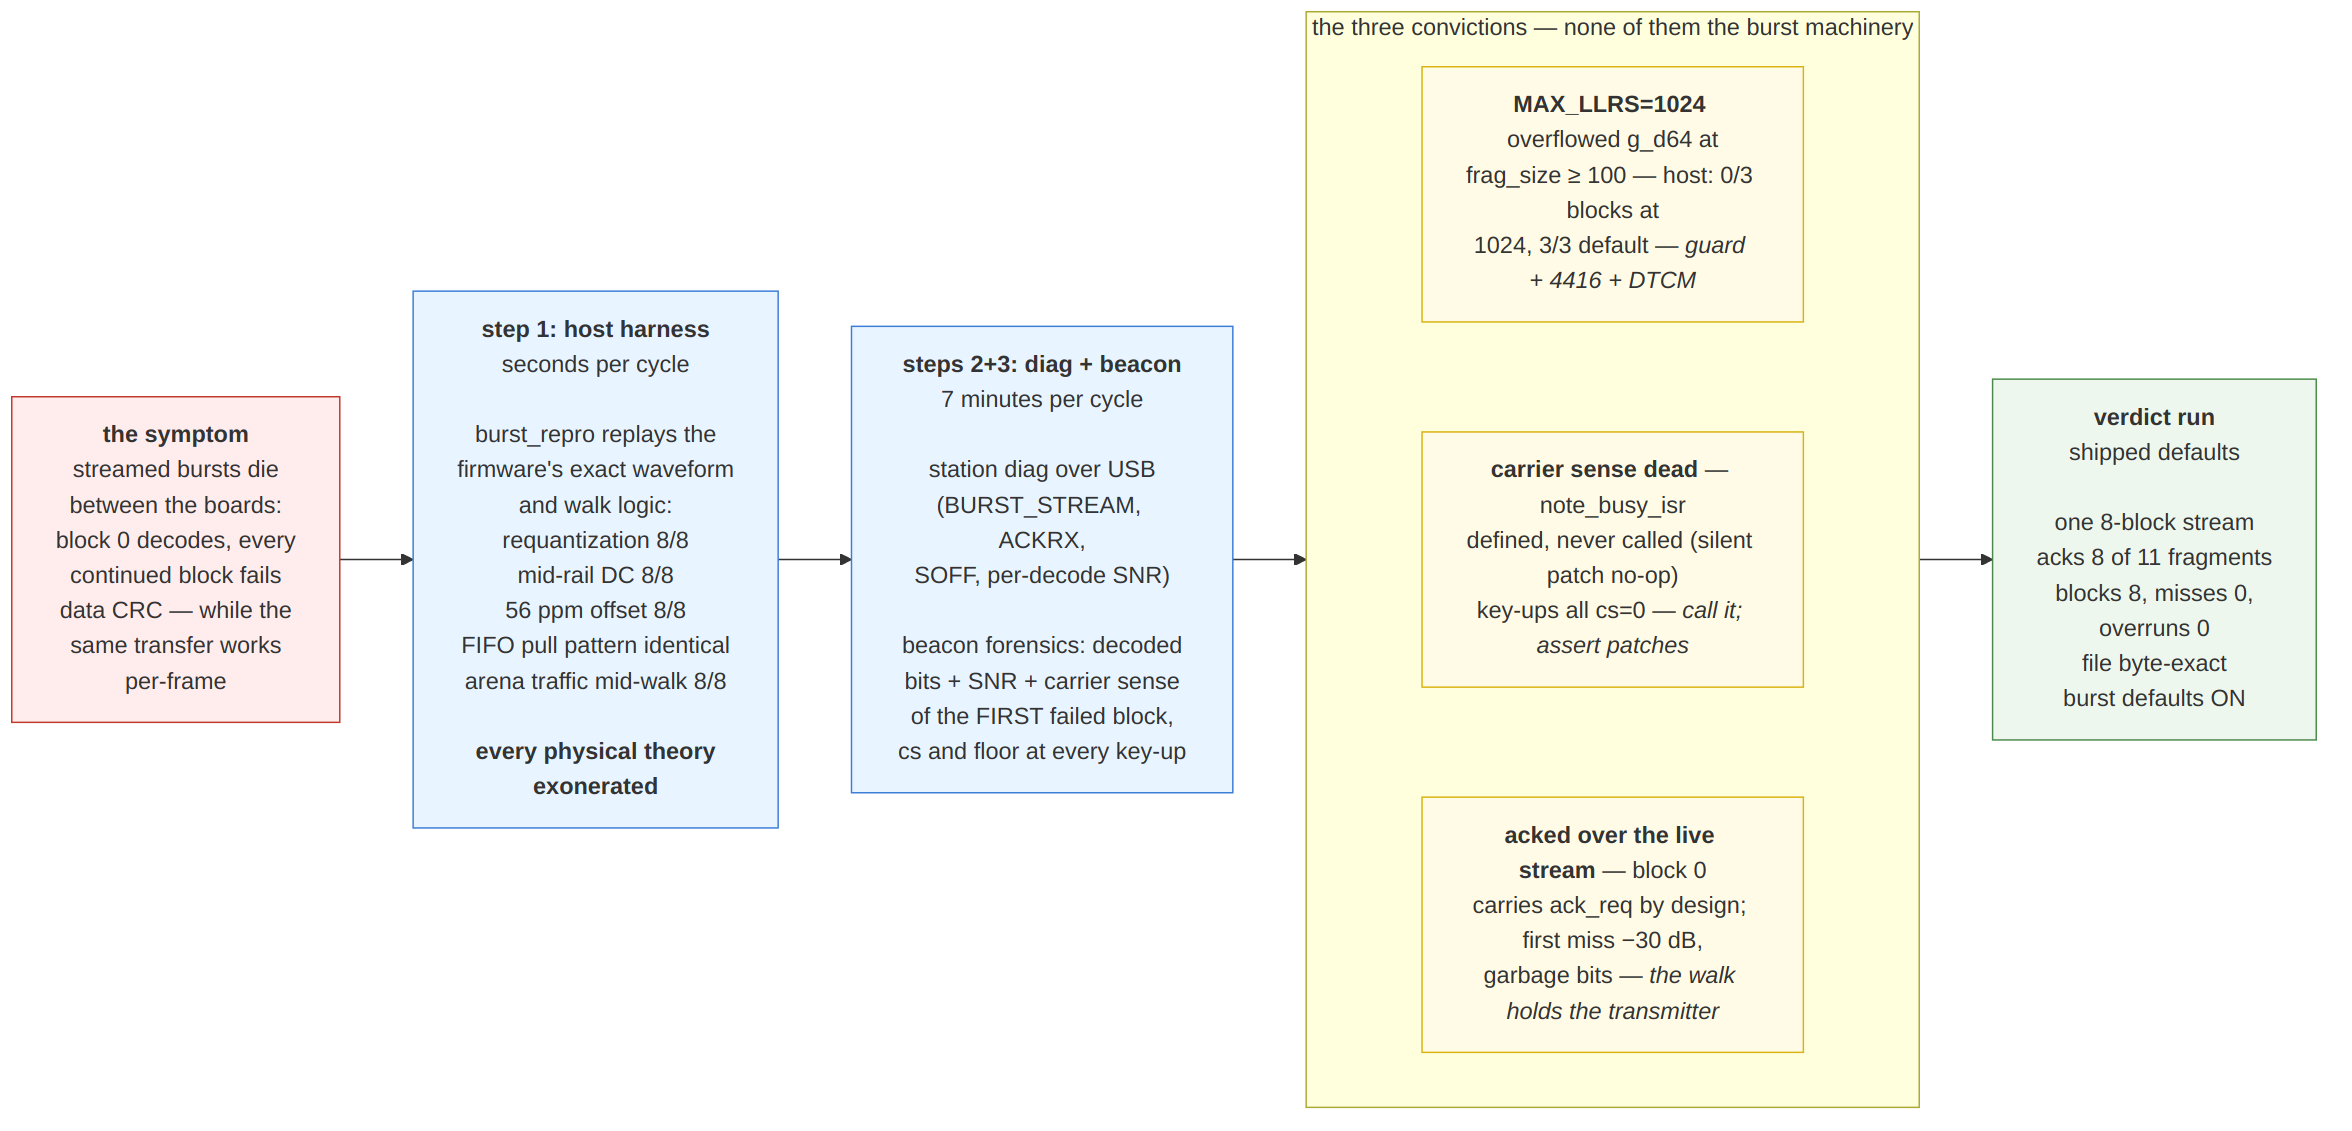
\includegraphics[width=\textwidth]{images/burst_debug.png}
    \caption{The diagnostic ladder. The host harness exonerates the
             physics before any board cycle is spent; the board-side
             instruments then carry the burden of proof, and each of the
             three convictions ends with a measured signature, not an
             argument.}
    \label{fig:burstdebug}
\end{figure}

\paragraph{Step 1: exonerate the physics.} A host harness
(\texttt{bench/burst\_repro.c}, \texttt{make burstrepro}) builds the
\emph{firmware's} streamed waveform --- station-style \texttt{EXT\_DATA}
blocks through the streaming generator --- and walks it with the
firmware's own burst logic, under the board's impairments applied one at
a time: the 12-bit DAC re-read by the 16-bit ADC at 3/4 scale, the
mid-rail DC offset, and a sample-rate offset between the ends. It
decoded 8 of 8 blocks under all of them at once, up to 56\,ppm ---
worse than the wire, whose $+0.01$\,Hz residual CFO puts the real
offset near 5\,ppm. It also replayed the DAC FIFO's exact
variable-sized pull pattern (sample-identical to a flat render) and
interleaved transmit-generator arena traffic mid-walk (harmless). Five
plausible theories died in one afternoon without touching a board, and
what remained was a certainty worth more than any of them: the bug was
in the firmware's \emph{interaction}, not in the shared DSP.

\paragraph{Steps 2 and 3: make the boards testify.} Two instruments
carried the rest. The station's diagnostic event stream
(\texttt{UP\_EVT\_DIAG}, readable from the host console) reports the
link layer's own decisions --- windows engaged, streams sent, bitmaps
received, streaming abandoned and why. And the firmware's beacon grew
\emph{forensic} fields: for the first failed continued block, the
decoded bits of its leading 44 bits (the LC word and sub-header are
predictable, so near-correct bits mean ``aligned but noisy'' while
garbage means the walk ran off the waveform), the SNR the demodulator
saw, and the carrier-sense level --- plus a recorder of the last four
transmitter key-ups with the carrier-sense mean and floor at each.
Reading them over JTAG needs neither a debugger halt nor
instrumentation in the signal path.

\paragraph{The three convictions.} None was the burst machinery.

\emph{First}, the radio build had inherited \texttt{-DMAX\_LLRS=1024}
from the small-frame bench images. A streamed block's LLR store is
sized by the padded symbol count, and any fragment size above roughly
100 bytes overflows \texttt{g\_d64} --- silently, because nothing
guarded it, and invisibly on the host, where the overflow lands in the
neighbouring receiver instance's rows and reads back self-consistently.
The harness convicted it cleanly: 0 of 3 blocks decode at 1024, 3 of 3
at the default. The receiver now \emph{refuses} a header whose
announced frame exceeds its buffers --- the header was valid; this
build cannot decode what it describes --- and the radio build sizes
\texttt{MAX\_LLRS} for the largest EXT frame, with the store placed in
DTCM by the linker script.

\emph{Second, carrier sense was dead} --- and had been since the commit
that claimed to move it into the converter tick. That patch defined the
tick-side function and never inserted the call: the scripted edit's
pattern had the wrong indentation, and a text replacement with no
assertion silently replaced nothing. The measured mean stayed zero,
\texttt{channel\_busy()} answered idle forever, and the commit's fix
had never run. The key-up recorder caught it in one glance ---
\texttt{cs=0} at every key-up, where a quiet wire reads about
$2\times10^4$, since the idle peer's DAC holds mid-rail. The repair is
one call; the lesson is a rule: every scripted patch replacement gets
an assertion.

\emph{Third}, the station answered block~0 \emph{over the top of the
rest of the stream}. A stream's first block carries the ack request on
purpose, so a peer that cannot stream still replies; with carrier
sense dead, nothing stopped the receiving board keying its bitmap ack
two seconds into the peer's 9.75\,s transmission --- and key-up drops
its own capture. The forensics showed precisely that: the first failed
block decoded at $-30$\,dB with garbage lead bits --- the signal was
simply gone --- while the transmitting board's counters showed a
complete, clean carrier. The structural fix does not lean on carrier
sense: a receiver whose walk still expects blocks holds its own
transmitter, with a deadline so a peer dying mid-stream cannot mute the
station forever. The ack then leaves when the walk ends, which is the
contract the link layer wanted all along.

\paragraph{The verdict run.} With all three fixes and \emph{no}
host-side configuration --- the burst defaults are now on --- one
8-block stream behind a single preamble acked 8 of 11 file fragments
in a single bitmap, the receiver's beacon read
\texttt{blocks 8, misses 0}, capture overruns and DAC underruns stayed
zero on both boards, and the 1200-byte incompressible file crossed
byte-exact. The 224-second-frame hazard that had earlier argued for
shipping bursts off (fragment size is fixed at engage, and a rung
collapse mid-transfer keeps sending fragments sized for the rung it
engaged at) turned out to be a symptom of these same bugs poisoning
the rate controller, not a property of the machinery.

The instruments outlived the hunt: the harness is a build target, the
beacon parser is a checked-in tool
(\texttt{bench/radio\_beacon.py}) whose field list lives in one place
beside the append-only beacon struct, and the triage ladder itself is
recorded where the next investigation will find it.

\subsection{A Sentinel on the Air}
\label{sec:cport_sentinel}

Calibrating the estimate fixed what the receiver \emph{measures}.  What
it reports when it has measured nothing took longer to find, because
every symptom pointed at the channel.

An ordinary two-board chat session, read afterwards from both consoles,
showed replies arriving 18--21\,s after they were queued on a wire
running at $+20$\,dB, interleaved with replies that arrived in one
second.  Both stations reported healthy counters, no timeouts and no
retransmissions.  The rung display made it worse: it read \texttt{rung
11} at attach and the very next frame went out at rung~0.

The instrumented exchange settles it in one screen.  Four messages,
75\,s apart, diagnostics on:

\begin{quote}\ttfamily\small
A 11:13:56 send "one" \ \ . rung 11 -> 0 (losses 0, cap 12)\ \ tx rung 0\\
B 11:14:15 << "one" \ \ \ \ . rung 11 -> 0 (losses 0, cap \ 0)\ \ tx rung 0\\
A 11:15:11 send "two" \ \ . rung \ 0 -> 11 (losses 0, cap 12)\ tx rung 11\\
B 11:15:12 << "two" \ \ \ \ . rung \ 0 -> 11 (losses 0, cap 12)\ tx rung 11\\
A 11:16:26 send "three" . (rung unchanged) \ \ \ \ \ tx rung 11\\
B 11:16:27 << "three" \ \ . rung 11 -> 0 (losses 0, cap \ 0)\ \ tx rung 0
\end{quote}

\texttt{losses 0} throughout, so no loss fallback; A's cap is 12
throughout, so A's view of the channel is correct.  B's cap collapses
to 0 on the exchanges whose gap exceeded 60\,s --- and 60\,s is
\texttt{SNR\_MAX\_AGE\_S}, the age at which the SNR filter empties.

The mechanism is three lines of arithmetic.  A frame's link-control
word carries \texttt{ctl\_filtered\_snr()} evaluated when the frame is
\emph{built}; with an empty history that function returns its
``no measurement'' sentinel, $-99$\,dB.  \texttt{lc\_pack} quantised
that as if it were a measurement, $\mathrm{rint}((-99+24)/2) = -38$,
and clamped it into the field's low rail, code~0.  The peer unpacked
code~0 as a genuine $-24$\,dB report, and \texttt{ctl\_tx\_rung} caps
the transmit rung by the peer's report: no rung's sensitivity clears
$-24$\,dB, so the cap became 0.  A station that had merely been quiet
for a minute was telling its peer \emph{``I hear you at $-24$\,dB''},
and the peer answered a one-byte acknowledgement with a 19-second
EXTREME frame.  Conversational pacing straddles 60\,s constantly, so
this was the common case rather than an edge: three of four replies in
the run above.

The repair is to give the field's code~0 the meaning it was already
carrying by accident.  Code~0 now means \emph{no measurement};
genuine reports occupy codes 1--15, $-22$ to $+6$\,dB, and a real
reading below the floor clamps to code~1 --- ``I hear you badly'' must
stay distinguishable from ``I have not heard you'', which is the entire
content of the bug.  \texttt{ctl\_tx\_rung} applies the report cap only
when a report exists; a peer that has genuinely gone away is still
handled by the request's staleness decay, which was doing that work all
along.  Choosing the code the old sentinel already clamped to makes the
change compatible in both directions: an unpatched sender's absent
measurement lands in code~0, so a patched receiver repairs the exchange
unilaterally, and an unpatched receiver reads code~0 exactly as it did
before.  (Argued from the encoding; both boards on the stand are
patched, so the mixed case is not measured.)

Re-running the identical script gives B's reply rungs as
$0, 11, 10$ where they were $0, 11, 0, 0$: acknowledgement air time
falls from $\approx$19\,s to $\approx$1\,s on every exchange that was
broken.  The one remaining slow frame is the first after twelve idle
minutes, which is the request's own decay and is intended.

Two displays were repaired with it, and the reason is not cosmetic.
The diagnostic printed \texttt{cap 0} for ``no report'' --- a cap of
zero and the absence of a cap rendered identically --- which is
precisely what made the defect expensive to read; it now prints
\texttt{no peer report -- request stands}.  And \texttt{status}
reported \texttt{stats.last\_rung}, the rung of the last frame actually
transmitted, which after an idle night is a memory rather than a state:
it is what read \texttt{rung 11} three seconds before transmitting at
rung~0.  The status frame now carries the rung the \emph{next} frame
would use, and the consoles show the last transmitted one only when the
two differ (\texttt{rung 0 (last tx 11)}).

The general lesson is worth more than the fix.  A sentinel encoded as a
number survives every layer that treats it as data: it printed as
$-99.0$\,dB in a status line, travelled the air as $-24$\,dB, and was
consumed by a control law that had no way to tell a measurement from
its absence.  The same day's audit turned up five instances of the same
shape --- the SNR display, the peer report, the $-10^{9}$ ``never''
timestamps, the cap, and this one, the only one that had escaped onto
the wire.  Where a quantity can be absent, absence needs its own
representation, and every consumer needs to be unable to mistake it for
a value.

\subsection{Broadcast on the Stand}
\label{sec:radio_bcast}

The broadcast design of Section~\ref{sec:cport_bcast} was verified on
the wire in two campaigns.  The first, a twelve-broadcast run at
rung~4, delivered 24 of 24 groups, and the campaign around it 38 of
39; the second put the block-statistics exchange on the boards.  What
each taught is recorded here, including a conclusion of the first
that the voice campaign later overturned.

\subsubsection{Pinning the one loss on the air, not the code}

The single missing group is worth the paragraph, because a whole group
vanishing looks exactly like a defect. It went \emph{whole}: not one
frame of it decoded, including the SYNC block that follows the
preamble. The host bench that answered the question builds the same
group with the \emph{same} firmware code and walks it with the same
\texttt{bc\_advance()} logic through the real streaming receiver
(\texttt{make bcrepro}, now part of the \texttt{make robust} gate); it
decodes 6/6 frames at rung~4 and 2/2 at rung~0, under the wire's
requantization, so the build-and-walk path was exonerated in seconds
rather than in seven-minute board cycles.

That left the air, and the beacon was extended to say so: an eight-deep
event ring recording every receiver event with its mode, type, packet
type, capture drops and position, and the loudest mean-square the
receiver heard while not transmitting. At the lost group the receiver
had heard a full-strength carrier ($1.15\times10^{8}$, against
$\sim$$2\times10^{4}$ for a quiet wire) with \emph{zero} capture-FIFO
drops, and had produced no event at all --- a missed acquisition, which
takes every frame behind it with it. That is the shape of every non-ARQ
loss, and it is the failure rate ARQ has been hiding all along by
retransmitting (Section~\ref{sec:cfo_unwrap} measured the same
thing from the other side, at $\sim$8\% of acquisitions before the
lag-$N$ unwrap fix). Broadcast cannot retransmit, which is precisely
why the EOS event reports what arrived.

That reading --- a missed acquisition on the air, nothing to fix --- was
wrong, and the report keeps it here because the evidence that
overturned it is instructive.  When the voice campaign of
\S\ref{sec:voice_onair} measured the same whole-group loss at
0.76\,\% per group on a clean wire, a host soak with no noise and no
boards (\texttt{make bcsoak}, \S\ref{sec:chan_harness}) reproduced it
deterministically: the streaming detector was committing an isolated
weak spike from a tone field \emph{entering} its window, two blocks
before the real preamble, and the failed attempts that followed
consumed the true peak, which the newest-block-only search never
revisits.  The beacon's ``full carrier, zero drops, no event'' is
exactly what that looks like from outside.  The commit gate that fixed
it is described there; whether the 1 in 39 of this campaign shared the
cause cannot be settled retroactively, but the mechanism was present
in the firmware that ran it.

\subsubsection{What the clean wire then taught}

Verifying the ported laws on the boards flushed out five real
firmware defects, one per run, each convicted by the boards' own
counters --- a sequence worth recording because every one masqueraded
as something else first:

\begin{itemize}
\item The \emph{sender was not listening on the mode it broadcasts
      in}: \texttt{follow\_rung} knew nothing about broadcast, the
      active-mode mask read EXTREME-only in the middle of a NORMAL
      broadcast, and every reply the receiver keyed was physically
      undecodable.
\item The reply window was anchored at EOB \emph{build} time,
      spending its first $\sim$2\,s on the EOB's own air; it arms at
      carrier drop now, sized $\sim$9.4\,s for the real chain (the
      peer's end-of-frame commit, its keying, the reply's air, our
      commit) after timestamps showed the receiver keying at :35
      against an expiry at :40.
\item The reply transport is pinned to the NORMAL floor --- BPSK~1/2
      decodes at any SNR the stream itself survives, and the desired
      rung rides inside the frame --- and the receiver logs
      \texttt{stats keyed}, which is what turned counter guesswork
      into comparable timelines.
\item After \emph{every} transmission of our own, the receivers are
      re-armed: the capture stream stitches pre-transmission samples
      to post, the detectors false-lock on the seam, and the re-arm
      skip blinds them for exactly the 1--4\,s in which a stats reply
      arrives. Twenty-two garbage-header events in one run; two of
      three replies lost. The chat link never noticed in a year of
      running, because its replies arrive seconds later.
\item The station must not key into a stats window the broadcast
      opened: a leftover chat frame in the window defeated every
      \emph{first} exchange while later ones worked --- which is
      precisely why it masqueraded as a timing race until the key-up
      recorder said otherwise.
\end{itemize}

The final clean run: three stats windows, three replies decoded within
1--2 seconds each, the deliberate rung-8 start re-rung to 12 in the
first window, and the file stored byte-identical. The fourth item is
the one with reach beyond broadcast: post-transmission receiver
blindness was latent in every half-duplex exchange this system runs,
and only a reply fast enough to land inside it could make it visible.

\subsection{Transfer Throughput: Two Levers, and Which One Mattered}
\label{sec:cport_levers}

The 13-minute transfer of the 68\,kB file that the capability
handshake enabled (\S\ref{sec:cport_caps}: 34 parts of 2\,kB, one
streamed window each) still ran at 66\% of the rung-12 channel rate,
and the per-part rhythm said where the rest was: each 2\,kB part went
out as \emph{three} acknowledgment cycles --- a window of eight, a
window of two, and a lone tail fragment. Two levers were measured
separately, on the same file and the same wire:

\begin{center}
\begin{tabular}{lccl}
\hline
 & time & rate & shape \\
\hline
baseline: 2\,kB parts, window 8 & 780\,s & 87\,B/s & 3 acks per part \\
window-aligned 1600\,B parts & 669\,s & 102\,B/s & 1 ack per part \\
window 16, parts \emph{not} re-aligned & 695\,s & 98\,B/s & tail penalty \\
aligned 3.2\,kB parts, window 16 & \textbf{596\,s} & \textbf{114\,B/s} & 1 ack per part \\
\hline
\end{tabular}
\end{center}

The first lever costs nothing: one console part is one station
message, so splitting parts at $\mathtt{win\_max} \times 200$ minus
the envelope head --- the peer's declared window, from the handshake
--- makes every message an exact multiple of the fragment and every
part exactly one acknowledgment. The third row is why this matters
more than window size, and it is the row worth remembering: a
\emph{bigger} window measured \emph{slower}, because the streamer
refuses short tails inside windows (deliberately --- a stream is
uniform blocks), so a misaligned part paid a whole extra ack cycle for
its 27-byte tail. Alignment first, capacity second.

The second lever buys the remainder with RAM nobody was using.
\texttt{BURST\_STREAM\_MAX} rose to 16 (a 26.2\,s window by the
builder's own sample count --- the air-time model in use at the time
said 25.3\,s and was later found 23\,\% short in general,
\S\ref{sec:cport_review}; the corrected figure is still under the
30\,s single-acknowledgment exposure cap) and messages to
3328 bytes --- and the memory to pay for it came from SRAM4, the one
region every earlier budget had left untouched. Its placement logic
inverts the usual instinct: SRAM4 sits in the D3 domain behind two bus
bridges, the \emph{slowest} RAM on the part, which makes it exactly
right for the station struct ($\sim$58\,kB with the larger pool) ---
touched at frame cadence from the main loop and never from the ISR.
Opening it took a linker region, a zero loop in startup (no RCC gate
exists for CPU access), and hoisting the 16-block stream buffer to
file scope so the linker could park its 33\,kB in D2 by name. After
the move: DTCM 56 of 128\,kB, AXI 496 of 512, D2 293 of 295, SRAM4 58
of 64 --- and ITCM's 64\,kB still the untouched reserve.

The final configuration moves the 68\,kB file in 9.9 minutes at
87\% of the raw channel rate, byte-exact, with three timeouts across
the hundred-odd windows of the measurement campaign and zero
retransmissions; what remains above the wire rate is preambles,
turnaround and carrier-sense gaps. One operational note carried into
the documentation: the \emph{first} bulk transfer to a stranger still
splits conservatively at window 8, because the handshake is triggered
by that very transfer --- its record arrives too late to size it. A
small bulk item sent first primes the record when the difference
matters.
